\documentclass[12pt, a4paper, openany]{report}
\def\VersionRapport{1.0}
\usepackage[utf8]{inputenc} % un package
\usepackage[T1]{fontenc}      % un second package
\usepackage[francais]{babel}  % un troisième package
\usepackage{layout}
\usepackage[top=2.7cm, bottom=2.5cm, left=3.5cm, right=3cm]{geometry}
\usepackage{setspace}
\frenchbsetup{StandardLists=true} % à inclure si on utilise \usepackage[french]{babel}
%\usepackage{enumitem}
\usepackage[shortlabels]{enumitem}
\usepackage{amssymb}
\usepackage{color}
\usepackage{listings}
\definecolor{dkgreen}{rgb}{0,0.6,0}
\definecolor{gray}{rgb}{0.5,0.5,0.5}
\definecolor{mauve}{rgb}{0.58,0,0.82}
\definecolor{rougecerise}{rgb}{0.73,0.043,0.043}
\lstset{frame=tb,
  language=Matlab,
  aboveskip=3mm,
  belowskip=3mm,
  showstringspaces=false,
  columns=flexible,
  basicstyle={\small\ttfamily},
  keywordstyle=\color{blue},
  commentstyle=\color{dkgreen},
  stringstyle=\color{mauve},
  breaklines=true,
  breakatwhitespace=true,
  tabsize=3,
  breaklines=true,
  morekeywords={matlab2tikz},
  morekeywords=[2]{1}, 
  keywordstyle=[2]{\color{black}},
  identifierstyle=\color{black},
  numbers=left,
  numberstyle={\tiny \color{black}},
  numbersep=9pt, 
  emph=[1]{for,end,break},
  emphstyle=[1]\color{red}
}
\usepackage{multirow} % pour les tableaux
\usepackage[table]{xcolor} % pour les tableaux
\usepackage{verbatim}
%\usepackage{subcaption}
\usepackage{graphicx}
\usepackage{moreverb}
\usepackage{url}
\usepackage{pst-all}
\usepackage{eso-pic,graphicx}
\usepackage{caption} 
\usepackage[colorlinks=true,urlcolor=blue,linkcolor=red]{hyperref}
\usepackage{array}
\usepackage[toc,page]{appendix}
\usepackage[off]{auto-pst-pdf}
\usepackage{hyperref} % pour le sommaire table des matières
\AddThinSpaceBeforeFootnotes % à insérer si on utilise \usepackage[french]{babel}
\FrenchFootnotes % à insérer si on utilise \usepackage[french]{babel}
\usepackage{fancyhdr}
\pagestyle{headings}
\usepackage{pifont}  %pour les puces
\usepackage{amsmath} %pour les puces
\usepackage{subfig}
\usepackage{verbatim} % pour le code en annexe 
%%%%%%%colones 
\newcolumntype{R}[1]{>{\raggedleft\arraybackslash }b{#1}}
\newcolumntype{L}[1]{>{\raggedright\arraybackslash }b{#1}}
\newcolumntype{C}[1]{>{\centering\arraybackslash }b{#1}}
%%%%%%% 
\renewcommand{\appendixpagename}{Annexes}
\renewcommand{\appendixtocname}{Annexes}
\title{Theme: Compte Rendu SLI 1}
\author{KHERBICHE \bsc{Ali}}
\date{2018-2019}
%new
\newcommand{\HRule}{\rule{\linewidth}{0.5mm}}

\begin{document}

%\selectlanguage{francais}
\pagenumbering{arabic} 
\makeatletter
\begin{titlepage}
\begin{sffamily}
\begin{center}
    % Upper part of the page. The '~' is needed because \\
    % only works if a paragraph has started.
    
\includegraphics[scale=0.5]{Logo_UT3.jpg}~\\[1cm]
    \textsc{\LARGE M1 ISTR-RODECO  }\\[1cm]
    \textsc{\Large Compte Rendu SLI 1}\\[1cm]
    % Title
    \HRule \\[0.4cm] % saut de ligne
    { \huge  \textsc {Travaux Pratiques 2 : Synthèse d'un Asservissement de Position par Retour d'Etat et Tachymetrique\\ Implémentation avec MATLAB/SIMULINK et RTW TARGET \\[0.4cm] }}

    \HRule \\[1cm]   % sous de ligne 
    
\includegraphics[scale=0.1]{logomaster.jpg}
    \\[1cm]
    % Author and supervisor
    \begin{minipage}{0.4\textwidth}
      \begin{flushleft} \large
         \textsc{\emph {Fait par:} \\KHERBICHE Ali}  
          \newline
          Promotion 2018-2019 \\
      \end{flushleft}
    \end{minipage}
    \begin{minipage}{0.4\textwidth}
      \begin{flushright} \large
        \emph{Tuteur et}
        \emph{Responsable de la Formation:} \textsc{M.Frédéric GOUAISBAUT}
      \end{flushright}
    \end{minipage}
    \vfill
    % Bottom of the page
    {\large Novembre 2018}
  \end{center}
  \end{sffamily}                
  \end{titlepage}  
\makeatother
   
%*********************** somaire **************
\renewcommand{\contentsname}{Sommaire}
\tableofcontents
%*********************** listes des figures **************
\listoffigures
%*********************** listes des tableaux **************
\listoftables

 \chapter*{Introduction}
	\addcontentsline{toc}{chapter}{Introduction}
	\paragraph{}
		Cette manipulation se propose de réaliser un asservissement de position en mettant en œuvre les techniques d’espace d’état continu. Le procédé utilisé est la platine ”asservissement de position" qui apparaît dans la \hyperref[fig1]{Figure 1}, déjà présentée dans les textes des manipulations des TP de licence EEA (2ème année) dont le principe est rappelé sur le schéma présenté dans la \hyperref[fig2]{Figure 2.}

	\begin{center}
	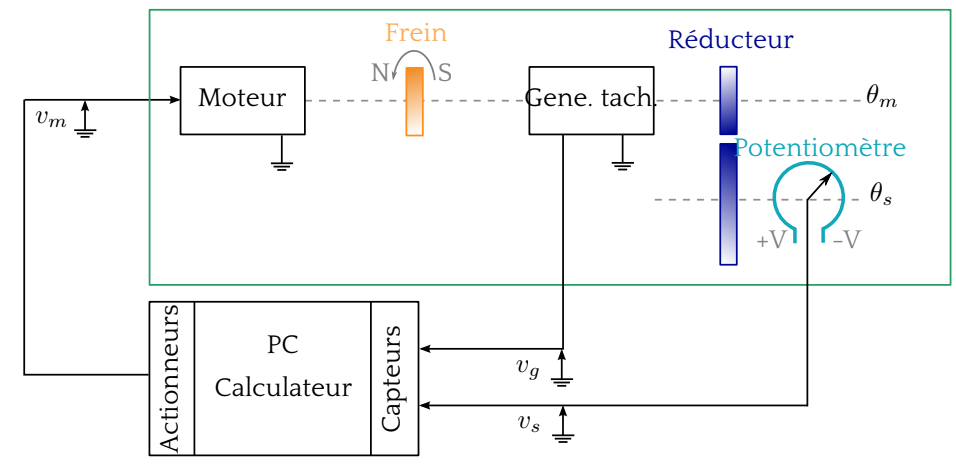
\includegraphics[scale=0.4]{schemamotor.png}
	\captionof{figure}{\textit{Asservissement de position par calculateur\\}}
	\label{fig1} 
	\end{center} 
	
	\begin{center}
	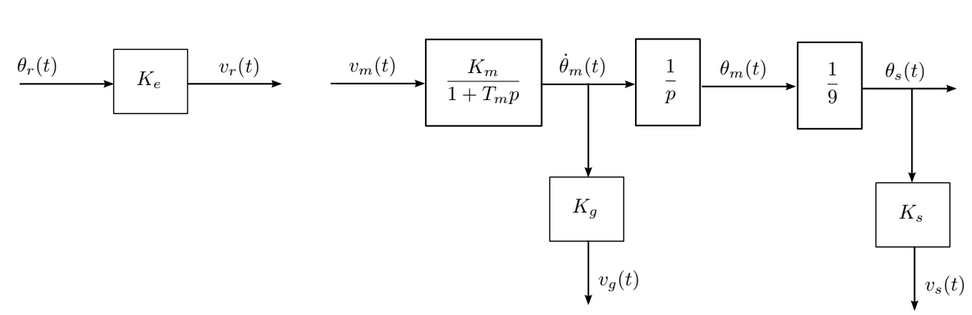
\includegraphics[scale=0.4]{schemablocmotor.png}
	\captionof{figure}{\textit{Eléments de la platine (asservissement de position)\\[4cm]}}
	\label{fig2} 
	\end{center}
	
	\begin{itemize} [label=\ding{70},font=\small \color{black}]
	\item $v_{m}(t)$\hspace{1mm} est la tension d'entrée du moteur.
	\item $\theta_{s}(t)$\hspace{1mm} est la position de l'axe secondaire du moteur.
	\item $\dot{\theta}_{m}(t)$ est la vitesse de rotation de l'axe principal du moteur.\\
	Les paramètres $K_{m}$ et $\tau_{m}$ seront déterminés dans la section XXX. Les coefficients commus sont $K_{e}$, $K_{s}$ et $K_{g}$, leur valeurs numériques sont données comme suit:
	\begin{itemize} [label=\ding{171},font=\small \color{black}]
	\item $K_{e} = 10(V.tr^{-1})$
	\item $K_{s} = 10(V.tr^{-1})$
	\item $K_{g} = 0.105(V.s.tr^{-1})$
	\end{itemize}
	\end{itemize}
	
	\paragraph{}
		Il est possible d’obtenir une mesure de $\theta_{s}(t)$ et de $\theta_{m}(t)$ via un potentiomètre et une génératrice tachymétrique.
		
		\begin{center}
		$v_{m}(t) = K_{s}\theta_{s}(t)$ \hspace{1.5cm} et \hspace{1.5cm} $v_{g}(t) = K_{g}\dot{\theta}_{m}(t)$ 
		\end{center}
		
 \chapter{Mise en place d'un retour d'état et d'un pré-compensateur}
	
	\section{Calcul du pré-compensteur}

	\paragraph{}
	Pour un système SISO (une entrée/une sortie) les pôles permettent de régler la dynamique du système, c’est-à-dire, le régime transitoire. Par contre, cette technique ne permet pas de régler le problème de la précision. Nous ne pouvons pas choisir le régime permanent du système en boucle fermée par le choix de K. Nous proposons une première structure de commande permettant d’assurer une erreur de position nulle en régime permanent tel que \cite{ref1} :
	
	\begin{center}
	$u(t) = -Kx(t) + Ny_{ref}(t)$ 
	\end{center}		

	où le pré-compensateur $N$ est un gain matriciel permettant de régler le gain statique du système en boucle fermée, avec:
	
	\begin{center}
	$N = \frac{1}{C(BK-A)^{-1}B}$ 
	\end{center}	
	Avec MATLAB\label{section 3.3} \hyperref[Annexe A]{voir Annexe A}, on a trouvé: $N= 1.389$
	
 %\input{chapitre2.tex}
 %\input{chap3.tex}
 %\input{chap4.tex}
\chapter*{Conclusion}
	\addcontentsline{toc}{chapter}{Conclusion}

\end{document}
